% =====================================================================
% International Journal of Greenhouse Gas Control (IJGGC) submission
% Elsevier elsarticle template. IJGGC uses the Harvard (author-date)
% reference system -> elsarticle-harv.bst + \citep / \citet (natbib).
% Draft format: "preprint" (single column). For final submission Elsevier
% recommends "review" (double-spaced) or a final layout (1p/3p/5p);
% the alternative styles (elsarticle-num / -num-names) are also shipped.
% The "authoryear" class option selects natbib author-date citations (\citet/\citep),
% required by IJGGC; without it elsarticle defaults to numbered citations.
% =====================================================================
\documentclass[preprint,authoryear,12pt]{elsarticle}

% Font setup
\usepackage[T1]{fontenc}
\usepackage{textcomp}

% Additional packages
\usepackage{graphicx}
\usepackage{float}
\usepackage{amsmath}
\usepackage{amssymb}
\usepackage{booktabs}
\usepackage{hyperref}
\usepackage{lineno}

\journal{International Journal of Greenhouse Gas Control}

\begin{document}

\begin{frontmatter}

\title{Modelling the depressurisation of CO$_2$ storage vessel at conditions
relevant for intermediate storage and transport}

% Authors (reused from the HydDown/blowdown paper; add co-authors as needed)
\author[ors]{Anders Andreasen\corref{cor1}}
\cortext[cor1]{Corresponding author}
\ead{anra@ors-consulting.com}
\address[ors]{ORS Consulting Aps, Borgergade 66 st th., DK-6700 Esbjerg, Denmark}

% TODO: highlights (3--5, max 85 chars each) - uncomment and fill:
% \begin{highlights}
% \item ...
% \end{highlights}

\begin{abstract}
% TODO: abstract
\end{abstract}

% TODO: keywords - uncomment and fill:
% \begin{keyword}
% CO$_2$ \sep depressurisation \sep dry ice \sep intermediate storage \sep transport
% \end{keyword}

\end{frontmatter}

\linenumbers

% =====================================================================
\section{Introduction}
\label{sec:introduction}
% TODO

% =====================================================================
\section{Experimental basis}
\label{sec:experimental}

The model is validated against two independent experimental campaigns which together span the
pressure range relevant for intermediate storage and transport of CO$_2$: the low- and
medium-pressure CARDICE experiments performed by Ineris in a 2\,m$^3$ sphere, and the
high-pressure, dense-phase experiments performed by SINTEF and NTNU in a small, densely
instrumented cylinder. The two campaigns are complementary. In the former the vessel reaches
the triple point and a large dry-ice bank is retained inside the vessel, whereas in the latter
the fluid starts in the dense-liquid region and flashes vigorously through the discharge nozzle.
Both datasets are openly available.

\subsection{CARDICE (Ineris 2\,m$^3$ sphere)}
\label{sec:exp-cardice}

The CARDICE (CARbon DIoxide iCE) Joint Industry Project comprises pilot-scale CO$_2$ blowdown
experiments carried out by Ineris in a 2\,m$^3$ steel sphere. The test matrix and a comparison
with the commercial tool Vessfire are reported by \citet{Vaillant2021}, while the rig,
instrumentation and calibration are documented in detail by \citet{Jamois2023}. The 1\,Hz
dataset is openly available \citep{CardiceData2024}.

The vessel is a sphere formed from two welded hemispheres, with an internal volume of
2.030\,m$^3$, an inner diameter of 1556\,mm and a mean wall thickness of 54\,mm. It is
fabricated from P355GH steel and rated for 200\,bara at $-60\,^\circ$C, with a total mass of
approximately 4.8\,t. The sphere is insulated with 100\,mm of rubber foam. A cooling
calorimetry test reported by \citet{Jamois2023} gives an overall external heat-transfer
conductance of 4.3\,W\,K$^{-1}$, equivalent to approximately 0.4\,W\,m$^{-2}$\,K$^{-1}$ over the
11\,m$^2$ outer surface. For the several-hour blowdowns this heat ingress is small relative to
the latent loads, so the process is effectively near-adiabatic.

CO$_2$ is released through a release pipe of 40\,mm inner diameter and approximately 2\,m
length, terminated by a calibrated orifice connected either to the middle of the sphere for a
vapour-space release or to the bottom for a liquid-space release. The measured quantities
comprise the absolute pressure in the sphere and in the release pipe, the fluid temperature at
six heights, the inner and outer wall temperatures at seven heights, the vessel mass of fluid
and solids from four load cells, and the mass flow rate through the release pipe. The load-cell
inventory, corroborated against the measured pressure and temperature, is used here as the
reference for the initial inventory and for the discharge calibration.

The pure-CO$_2$ tests are numbers 5 to 10; the sphere was filled with liquid to approximately
the middle. Three initial pressure levels are each realised as a vapour-space (gas) release and
a liquid-space (liquid) release, as summarised in Table~\ref{tab:cardice-matrix}. The gas
releases produce a large retained dry-ice bank inside the sphere, whereas the liquid releases
leave essentially no solid inside the vessel; the dry ice a liquid release produces forms
downstream of the orifice instead.

\begin{table}[htbp]
\centering
\caption{CARDICE pure-CO$_2$ test matrix. $P_0$ and $T_0$ are the initial pressure and
temperature. The orifice diameter for test~8 is an effective value (Section~\ref{sec:discharge}).}
\label{tab:cardice-matrix}
\begin{tabular}{llccc}
\toprule
Test & Release & $P_0$ (bar) & $T_0$ ($^\circ$C) & Orifice (mm) \\
\midrule
5  & Gas    & 20 & $-20$ & 3 \\
6  & Liquid & 20 & $-20$ & 3 \\
7  & Gas    & 15 & $-29$ & 4 \\
8  & Liquid & 15 & $-29$ & 5$^{*}$ \\
9  & Gas    & 10 & $-40$ & 4 \\
10 & Liquid & 10 & $-40$ & 4 \\
\bottomrule
\end{tabular}
\end{table}

\subsection{Dense-phase experiments (SINTEF)}
\label{sec:exp-sintef}

The second campaign consists of the dense-phase depressurisation experiments performed by
SINTEF Energy Research and NTNU in the ECCSEL facility \citep{Hoydalsvik2026}. Relative to
CARDICE these experiments probe a very different part of the operating envelope, namely a
high-pressure ($\sim$120\,bar), sub-cooled dense-liquid initial state, and the fluid flashes
strongly through the discharge nozzle. The open dataset accompanies the paper.

The vessel is a vertical stainless-steel (SS316) cylinder of 273\,mm inner diameter and
1000\,mm internal height ($\sim$0.058\,m$^3$), with a 25.4\,mm wall, a 50\,mm bottom plate and
an 80\,mm lid, rated for 138\,bar and insulated with 50\,mm of Armaflex LTD. It is densely
instrumented with 26 thermocouples (fluid and wall temperatures at six heights, with four
radial positions per height: fluid on the central axis, fluid 5.5\,mm from the wall, wall 3\,mm
inside the inner surface, and the outer wall), together with four Keller pressure
transducers and three scales for the vessel weight. The vessel pressure is taken as the mean of
the transducers mounted 170\,mm from the top and 50\,mm from the bottom; two further transducers
measure the pressure immediately before and at the nozzle throat. The raw signals are sampled at
1\,kHz and averaged to 0.5\,Hz.

CO$_2$ is discharged through an interchangeable converging nozzle of throat diameter 8.0, 6.5 or
4.5\,mm (inlet diameter 32\,mm, half-angle $60^\circ$) in one of two configurations: directly
through an opening at the top of the vessel (no riser, a vapour-space release), or through a
20\,mm riser tube drawing liquid from 9\,mm above the floor (a liquid-space release). The nine
pure-CO$_2$ tests used here (three without a riser and six with) are summarised in
Table~\ref{tab:sintef-matrix}. As for CARDICE, the no-riser (gas) releases retain a small
in-vessel dry-ice bank, whereas the riser (liquid) releases drain and empty before the triple
point is reached.

\begin{table}[htbp]
\centering
\caption{SINTEF dense-phase pure-CO$_2$ test matrix. $P_0$ and $T_0$ are the initial pressure
and temperature; the configuration denotes a top opening (no riser, gas) or a bottom riser tube
(liquid).}
\label{tab:sintef-matrix}
\begin{tabular}{lcccl}
\toprule
Test & $P_0$ (bar) & $T_0$ ($^\circ$C) & Nozzle (mm) & Configuration \\
\midrule
Exp71 & 122.6 & 25.2 & 8.0 & No riser (gas) \\
Exp72 & 119.0 & 24.9 & 6.5 & No riser (gas) \\
Exp75 & 119.0 & 25.0 & 4.5 & No riser (gas) \\
Exp52 & 119.9 & 15.4 & 8.0 & Riser (liquid) \\
Exp53 & 119.5 & 24.4 & 8.0 & Riser (liquid) \\
Exp56 & 119.1 & 15.2 & 6.5 & Riser (liquid) \\
Exp57 & 116.8 & 24.5 & 6.5 & Riser (liquid) \\
Exp45 & 119.9 & 14.5 & 4.5 & Riser (liquid) \\
Exp46 & 116.7 & 24.4 & 4.5 & Riser (liquid) \\
\bottomrule
\end{tabular}
\end{table}

% =====================================================================
\section{Model}
\label{sec:model}
% TODO

\subsection{Thermodynamics and the solid-CO$_2$ lever}
\label{sec:thermo}
% TODO: all-CoolProp fluid (imposed-phase extrapolation below the triple point)
% + precomputed solid-CO2 property table; lever-rule flashes.

\subsection{Discharge model}
\label{sec:discharge}
% TODO: HEM rate with a solid-aware throat; non-equilibrium (HNE) liquid boost;
% phase-split discharge coefficients.

\subsection{In-vessel dry-ice formation}
\label{sec:dryice}
% TODO: two-zone triple-point plateau and sublimation descent; atmospheric lever.

\subsection{Heat and mass transfer}
\label{sec:heat}
% TODO: two-node wall; Churchill-Chu gas wall; Cooper/Rohsenow boiling;
% sublimation-tracking dry-ice wall.

% =====================================================================
\section{Results and validation}
\label{sec:results}

The model is applied to all fifteen experiments described in Section~\ref{sec:experimental}
using the sub-models of Section~\ref{sec:model}. For each case the initial liquid level is
calibrated to the measured load-cell inventory, and the orifice discharge coefficient and, for
liquid releases, the non-equilibrium factor are set as described in
Section~\ref{sec:discharge}. The measured traces are time-shifted to the model: the gas
releases, which decline in pressure from the onset, are anchored at a mid-blowdown reference
pressure, whereas the slow liquid drains are anchored on the onset of the inventory decline.
Below the triple point the gas-contact wall uses the Churchill--Chu free-convection coefficient
and the wetted wall the Cooper boiling correlation (Section~\ref{sec:heat}).

\subsection{Low- and medium-pressure blowdown (CARDICE)}
\label{sec:results-cardice}

The central experimental contrast, a large retained dry-ice bank for the gas releases and
essentially none for the liquid releases, is reproduced across the whole set.
Table~\ref{tab:cardice-results} compares the modelled and measured initial inventory, retained
dry ice and minimum wetted-wall temperature.

\begin{table}[htbp]
\centering
\caption{CARDICE model predictions compared with measurements: initial inventory $m_0$,
retained in-vessel dry ice, and minimum wetted (bottom) wall temperature.}
\label{tab:cardice-results}
\begin{tabular}{llccc}
\toprule
 & & $m_0$ (kg) & Retained dry ice (kg) & Wetted-wall min ($^\circ$C) \\
Test & Phase & model/meas. & model/meas. & model/meas. \\
\midrule
5  & Gas    & 824 / 823 & 266 / 217 & $-78$ / $-75$ \\
6  & Liquid & 804 / 802 & 0 / 4.2   & $-24$ / $-24$ \\
7  & Gas    & 790 / 791 & 302 / 298 & $-76$ / $-75$ \\
8  & Liquid & 761 / 758 & 0 / 3.8   & $-32$ / $-32$ \\
9  & Gas    & 904 / 904 & 392 / 412 & $-72$ / $-75$ \\
10 & Liquid & 745 / 743 & 0 / 5.1   & $-42$ / $-40$ \\
\bottomrule
\end{tabular}
\end{table}

For the gas releases (tests 5, 7 and 9) the model retains 266, 302 and 392\,kg of in-vessel dry
ice against measured values of 217, 298 and 412\,kg. The agreement is best for test 7, where
the retained mass is reproduced to within 2\%; test 5 is over-predicted and test 9 slightly
under-predicted. The over-prediction for test 5 is consistent with its wall sensible-heat store,
which sets the sublimation load and which the lumped wall description cannot resolve spatially.
In each case the blowdown follows the observed three-stage behaviour (an initial gas/liquid
depressurisation, a multi-hour pressure plateau at the triple point while the liquid freezes,
and a final gas/solid sublimation descent), and the wetted (bottom) wall cools to
approximately $-75\,^\circ$C, in agreement with the coldest measured sensors. The comparison for
test~7 is shown in Figure~\ref{fig:cardice-t7}.

\begin{figure}[htbp]
\centering
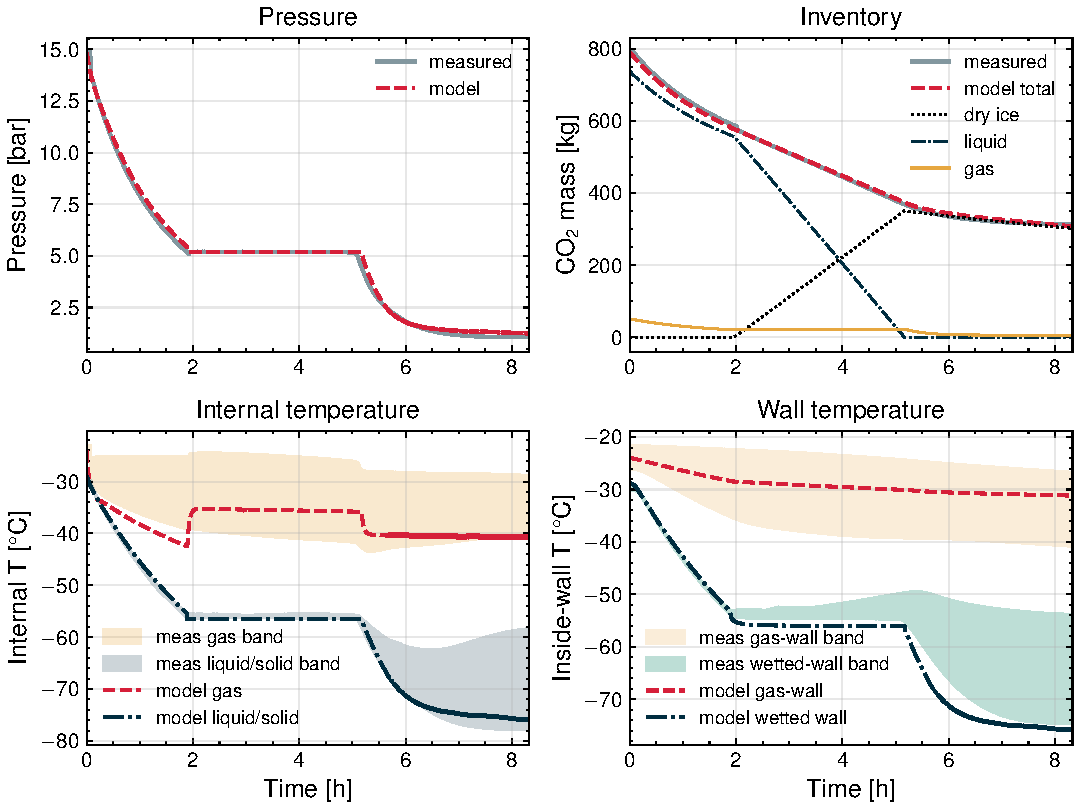
\includegraphics[width=\textwidth]{figures/cardice_t7}
\caption{CARDICE test~7 (gas release, 15\,bar): model (dashed) versus measured 1\,Hz data.
Panels show the vessel pressure, the inventory with the modelled gas/liquid/solid breakdown, the
internal fluid temperature (measured upper and lower bands versus the modelled gas and
liquid/solid temperatures), and the inside-wall temperature (measured bands versus the modelled
gas-contact and wetted-wall nodes).}
\label{fig:cardice-t7}
\end{figure}

The liquid releases (tests 6, 8 and 10) drain and boil out before the vessel reaches the triple
point and retain essentially no solid inside the vessel. The model reproduces this, emptying to
a small residual gas heel rather than the measured 4--5\,kg. The pressure and inventory
histories are captured well; Figure~\ref{fig:cardice-t8} shows test~8, for which the modelled
liquid drain and the time to empty match the data.

\begin{figure}[htbp]
\centering
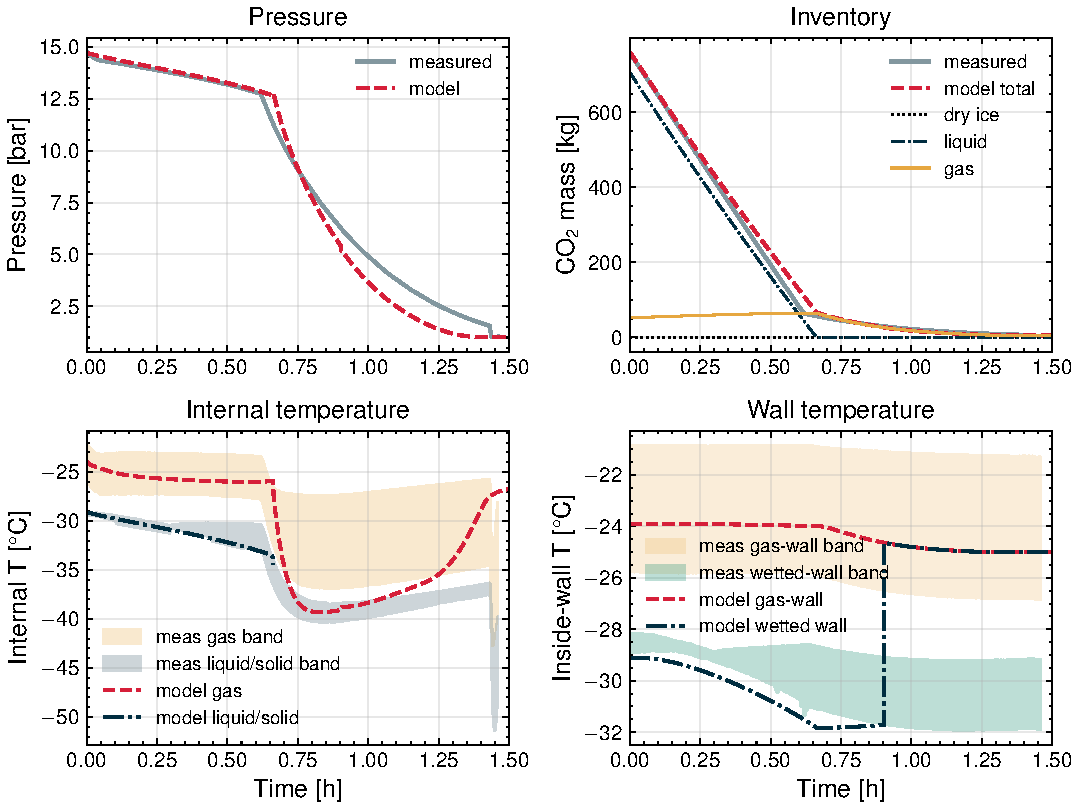
\includegraphics[width=\textwidth]{figures/cardice_t8}
\caption{CARDICE test~8 (liquid release, 15\,bar): model (dashed) versus measured 1\,Hz data,
panels as in Figure~\ref{fig:cardice-t7}. The liquid drains and boils out before the triple
point, leaving essentially no in-vessel dry ice.}
\label{fig:cardice-t8}
\end{figure}

The principal discrepancy is the bulk gas temperature for the gas releases, which the
zero-dimensional model under-predicts relative to the warm upper region of the vessel. The real
vapour is strongly stratified, warm near the top and cold near the interface, which a
single well-mixed gas node cannot represent, as it returns an average and mixes in cold
boil-off vapour. This is a fundamental limitation of the lumped description rather than a
heat-transfer deficiency, and the same behaviour is reported for the zero-dimensional tool
Vessfire \citep{Vaillant2021}.

\subsection{Dense-phase blowdown (SINTEF)}
\label{sec:results-dense}

The dense-phase experiments start as a sub-cooled liquid at approximately 120\,bar and flash
into the two-phase region during the initial, rapid depressurisation. As for CARDICE, the
no-riser (gas) and riser (liquid) configurations behave very differently, and both are
reproduced.

For the no-riser (gas) releases the dense liquid remains in the vessel, cools to the triple
point and freezes. The model retains approximately 8.4, 7.8 and 8.1\,kg of dry ice for Exp71,
Exp72 and Exp75, in close agreement with the measured value of approximately 8.4\,kg for Exp71.
The comparison for Exp72 is shown in Figure~\ref{fig:munke-exp72}.

\begin{figure}[htbp]
\centering
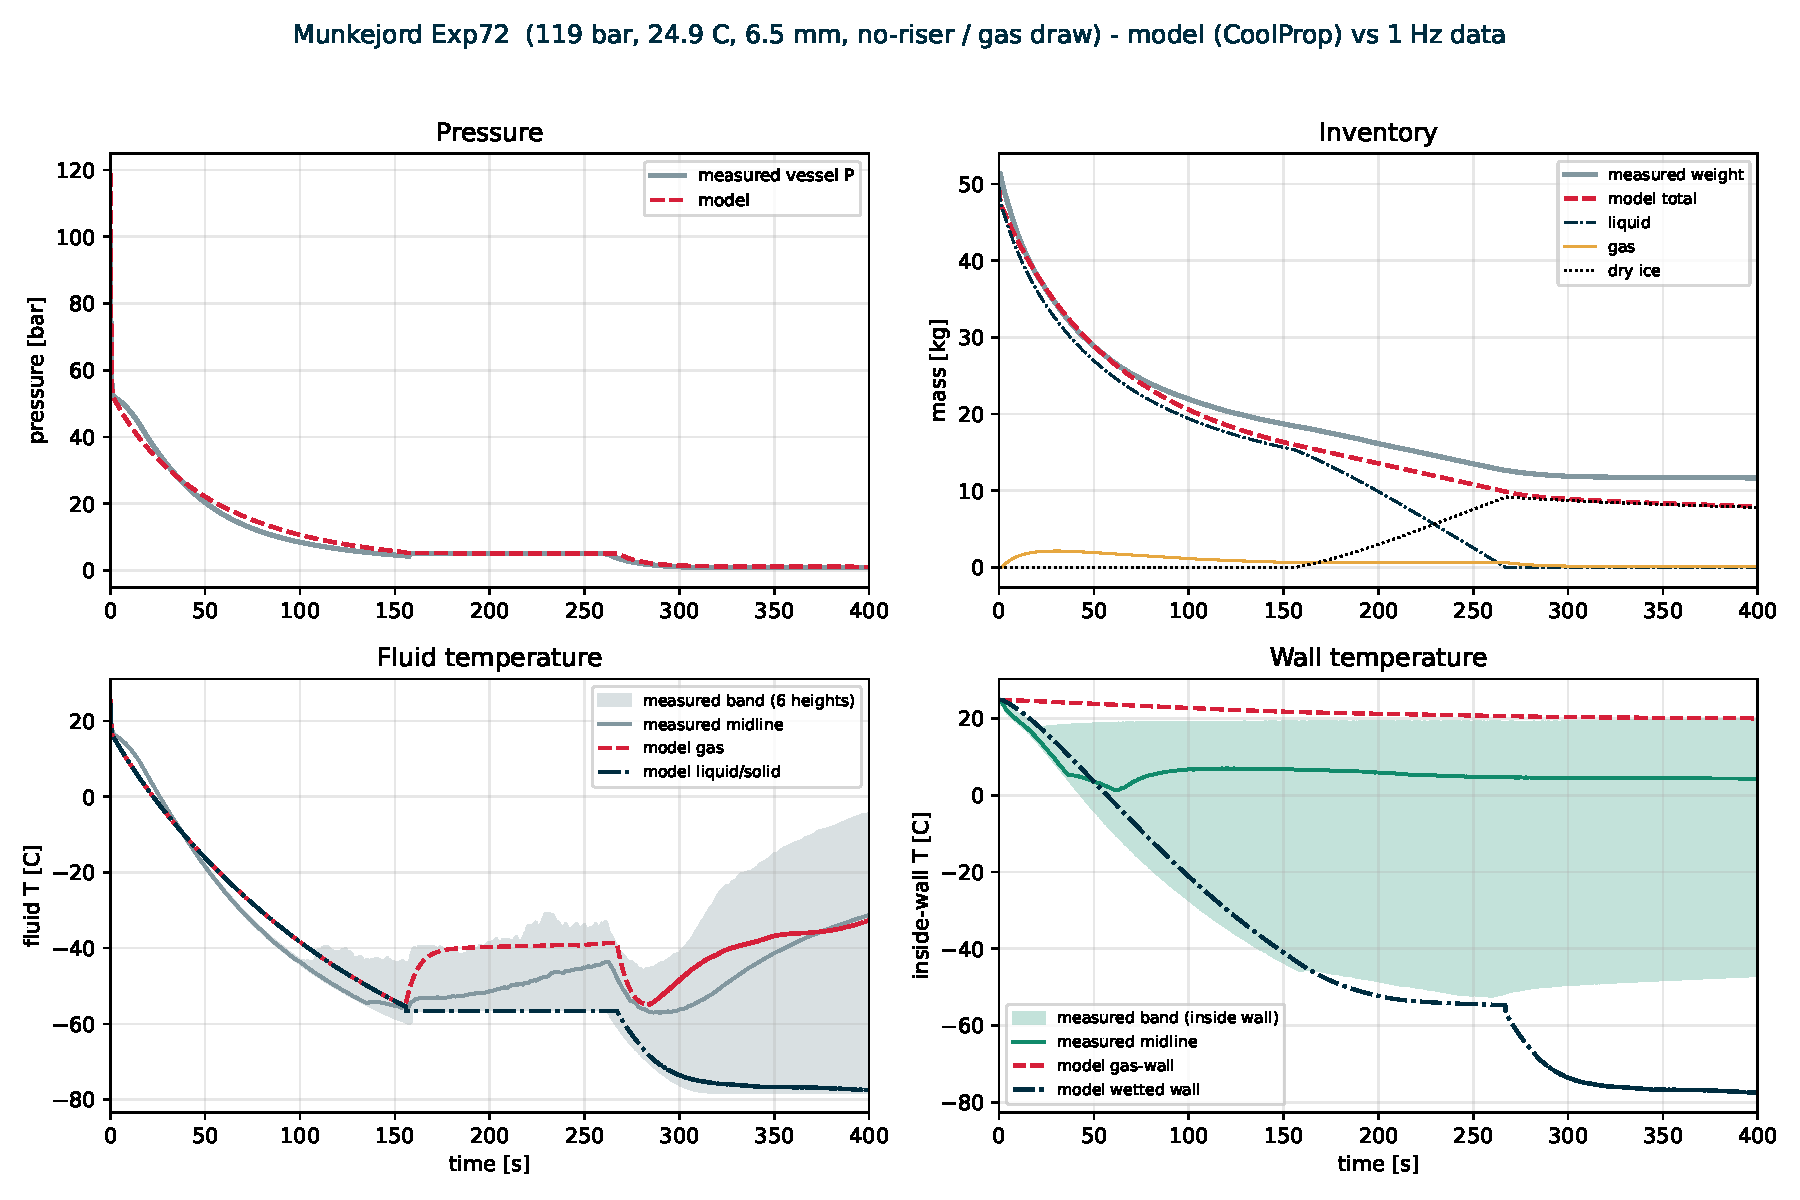
\includegraphics[width=\textwidth]{figures/munke_exp72}
\caption{SINTEF Exp72 (no-riser gas release, 119\,bar, 6.5\,mm nozzle): model (dashed) versus
measured data. Panels as in Figure~\ref{fig:cardice-t7}. The dense liquid remains in the vessel,
cools to the triple point and forms a retained dry-ice bank.}
\label{fig:munke-exp72}
\end{figure}

For the riser (liquid) releases the vessel drains through the riser and empties before the
triple point, leaving no in-vessel solid, as observed. The rapid dense-phase depressurisation
is captured well: the pressure falls from approximately 120\,bar, flashes onto the two-phase
saturation line at approximately 52\,bar, and follows the measured decline closely, while the
modelled gas and liquid/solid temperatures bracket the measured stratification band. The
comparison for Exp53 is shown in Figure~\ref{fig:munke-exp53}.

\begin{figure}[htbp]
\centering
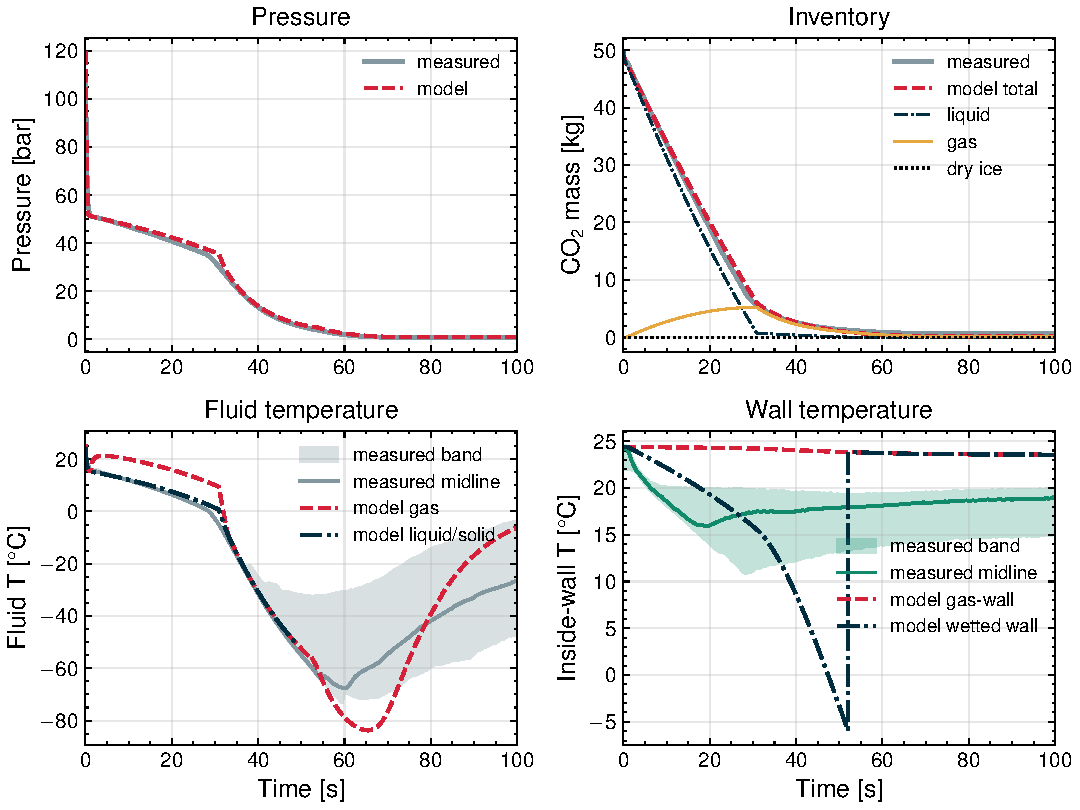
\includegraphics[width=\textwidth]{figures/munke_exp53}
\caption{SINTEF Exp53 (riser liquid release, 119.5\,bar, 8.0\,mm nozzle): model (dashed) versus
measured data. Panels as in Figure~\ref{fig:cardice-t7}. The vessel drains through the riser and
empties before the triple point; the first 100\,s, covering the active blowdown, are shown.}
\label{fig:munke-exp53}
\end{figure}

Two limitations are noted for the dense-phase cases. As for CARDICE, the bulk gas temperature
reflects the well-mixed assumption and does not resolve the vertical stratification observed in
the fluid thermocouples. In addition, in the gas/solid tail of the no-riser cases the modelled
dry-ice-contact wall tracks the sublimation temperature and reads colder than the measurements;
the relatively thick wall and the thin ice layer in these experiments allow lateral conduction
in the wall to re-warm the ice-contact metal, an effect a one-dimensional wall treatment does
not capture.

% =====================================================================
\section{Discussion}
\label{sec:discussion}
% TODO: 0-D limitations (stratification), model choices, applicability.

% =====================================================================
\section{Conclusions}
\label{sec:conclusions}
% TODO

% =====================================================================
\section*{CRediT authorship contribution statement}
% TODO

\section*{Declaration of competing interest}
% TODO

\section*{Acknowledgements}
% TODO

% =====================================================================
\bibliographystyle{elsarticle-harv}
\bibliography{references}

\end{document}
